\documentclass[a4paper,11pt]{article}
%\documentclass[a4paper,9pt,landscape]{article}
\usepackage[english]{babel}
%\usepackage[utf8]{inputenc}
\usepackage{graphicx}
\usepackage{fullpage}
\usepackage{amsmath}
\usepackage{pdfpages}
\usepackage{listings}
\usepackage{color}
\usepackage{multicol}
\usepackage{fancyhdr}
\usepackage[top=1.5cm, bottom=4cm, left=2.5cm, right=2.5cm]{geometry}
\usepackage{hyperref}
\usepackage{verbatim}
\setlength{\voffset}{-9pt}
%\setlength{\hoffset}{-1in}
%\setlength{\marginparsep}{0.5cm}


\setlength{\parindent}{1cm}
%\setlength{\parskip}{-0.1cm}
%\setlength{\columnseprule}{0.4pt}
\setlength{\footskip}{0.5cm}
\setlength{\headheight}{15pt}
\setlength{\headsep}{2cm}

\fancypagestyle{tcr}{%
  \fancyhf{} %clear all headers and footers fields
  \fancyhead[R]{\thepage}
  \fancyhead[L]{\textbf{Lab No 5 TDDC78}}
  \renewcommand{\headrulewidth}{0.4pt}
}

\definecolor{dkgreen}{rgb}{0,0.6,0}
\definecolor{gray}{rgb}{0.5,0.5,0.5}
\definecolor{mauve}{rgb}{0.58,0,0.82}
\lstset{
  title=\lstname,
  frame=t,
  %aboveskip=-0.5cm, 
  %belowskip=0pt,
  basicstyle=\footnotesize\ttfamily,
  keywordstyle=\color{blue},          % keyword style
  commentstyle=\color{dkgreen},       % comment style
  stringstyle=\color{mauve},         % string literal style
  showstringspaces=false,         % underline spaces within strings
  tabsize=2,
  language=C,
  title=\caption,
  %xleftmargin=-1cm
}


\begin{document}
%% title stuff
\title{Lab No 5 TDDC78}
\author{Linus Mellberg (linme560) \and Oskar Aagaard (oskaa489)}
\date{\today}
\maketitle
\pagebreak
%\setcounter{page}{1}
%\begin{multicols}{2}
\thispagestyle{tcr}
\pagestyle{tcr}
%\tableofcontents

\section{Tools}
This assignment is to test some of the debugging tools available for debugging parallel programs.
A good understanding of this type of program is useful for effectively debugging and developing parallel programs.

\subsection{ITAC/Traceanalyzer}
The program in assignment 4 was used to try the ITAC/traceanalyzer tool.
This tool is used to do profiling and tracing in parallel programs.
To trace our program we wanted to see when the collision analysis is done, when the program is communicating and how the pressure is changing over time.
The changes needed to be done in the program was to mark the section where the collisions are computed and add a counter for the pressure.
The doesn't count the actual pressure but instead the total momentum that has been transferred to the walls.
This value should increase linearly.

After the first run the load seemed to be a bit uneven especially in the beginning of the execution.
We chose to add another counter on the number of particles on each process.
The result can be seen in \ref{bug}.
The particles first moves to half of the processes and after a while they spread evenly to the processes.
This is not expected, the particles should be evenly distributed all the time.
The code was examined and it was found that there were a bug in the initialization of the particles.
They all had positive velocity in the vertical direction.
The bug was fixed and the both the particle distribution and the load balancing became better.
The number of particle chart can be seen in \ref{correct}.

The chart that shows how the program execution is divided over time can be seen in \ref{timeline}.
Just a few timesteps of the execution is shown as the chart is unreadable when everything is shown.
The MPI calls are red, the collision analysis is light blue and the rest of the code is dark blue.
As expected most of the execution time is spent int the collision analysis.
The time spent sending data is very low, but because of some load imbalance faster processes has to wait at the end of each timestep.
This does not seem to be because of a slow data transfer, the problem is that the slower processes isn't ready to send data yet.
The slowest process, which can send and recieve data immediately, has an MPI call that is so fast it can't be seen in the chart.

Figure \ref{quantitative} shows the quantitative chart.
This shows how many processes that are doing a certain thing at a point in time.
Most of the area in this graph is covered by collision analysis code.
There is also a little part of the area that is used by processes waiting to send or recieve data.
All other calculations are negligible.
The load balancing is alright and the most of the computing time is spent in the collision analysis code.

Figure \ref{pressure} shows how the pressure develops over time.
8 processes are used and the layout of the grid is $2\times4$.
This means that the corner processes will have three times as much wall as the processes in the middle.
\begin{center}
  \begin{tabular}[h]{|l|l|l|l|}
    \hline
    &   &   &  \\[2ex]
    \hline
    &   &   &  \\[2ex]
    \hline
  \end{tabular}
\end{center}
This can be seen in the chart as the pressure for four of the processes grows three times faster than the rest of them.

\begin{figure}[!h]
  \caption{Number of particles on each node with bug.}
  \label{bug}
  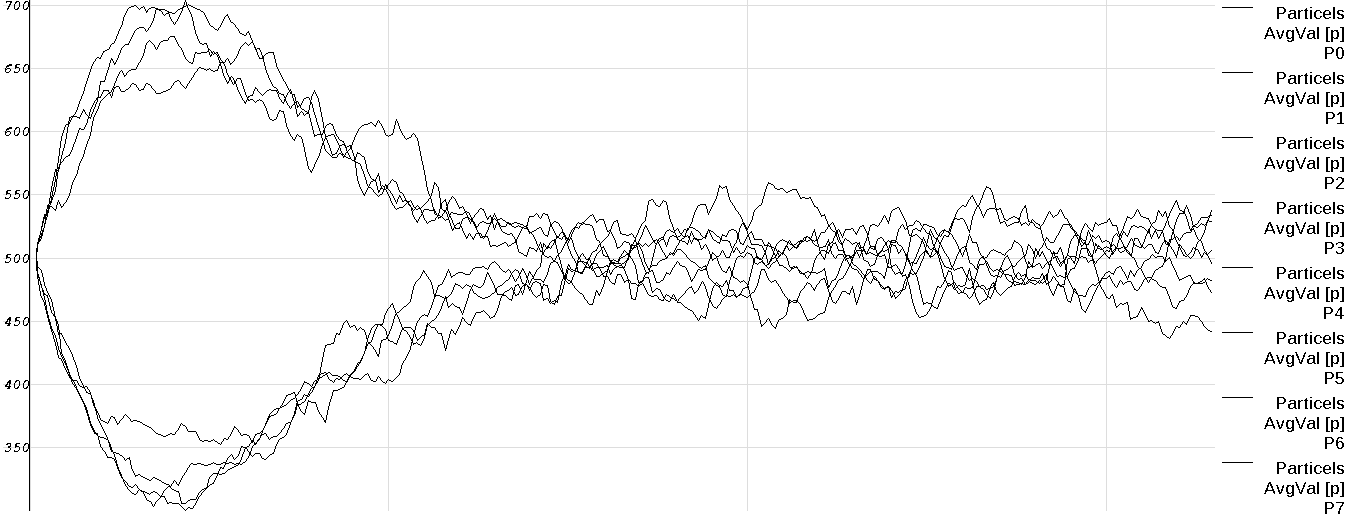
\includegraphics[width=15cm]{chart_no_particles_bug.png}
\end{figure}

\begin{figure}[!h]
  \caption{Number of particles on each node, correct program.}
  \label{correct}
  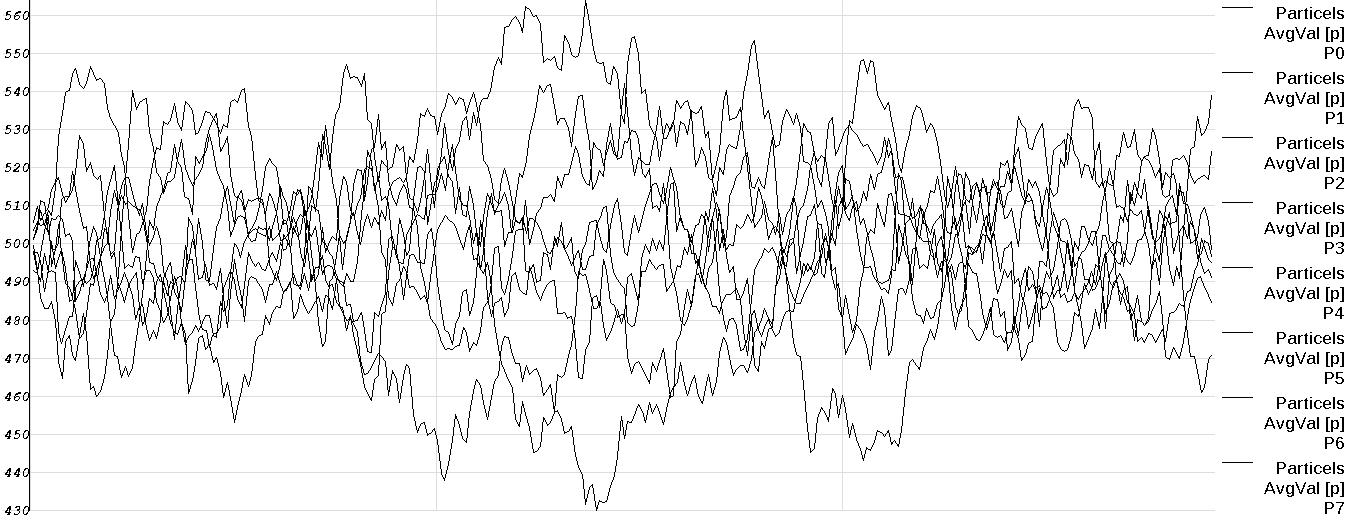
\includegraphics[width=15cm]{chart_no_particles_correct.png}
\end{figure}

\begin{figure}[!h]
  \caption{Timeline chart of a few timesteps.}
  \label{timeline}
  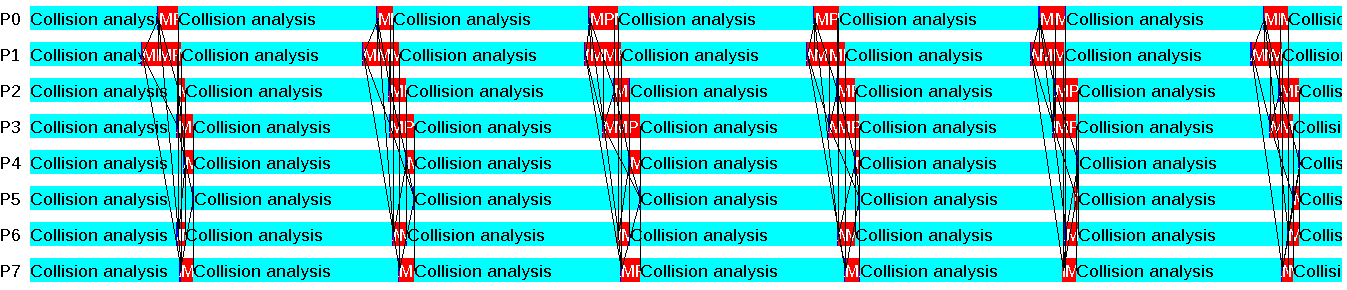
\includegraphics[width=15cm]{chart_load_balance.png}
\end{figure}

\begin{figure}[!h]
  \caption{Quantitative chart demonstrating load balance.}
  \label{quantitive}
  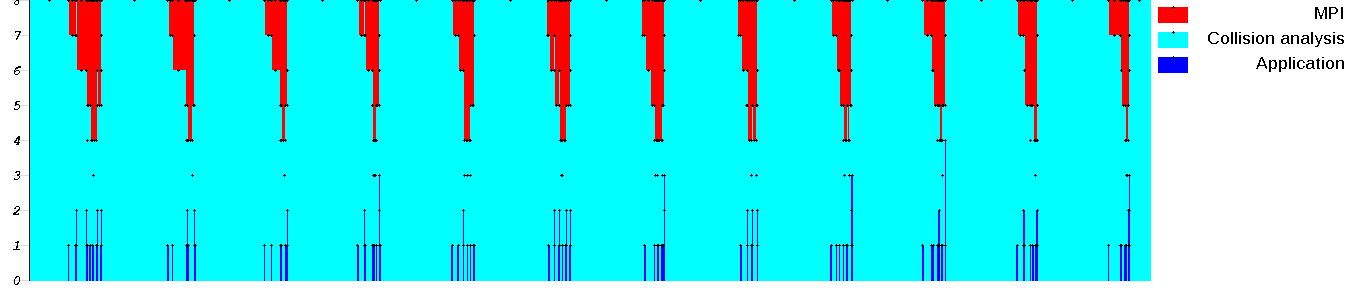
\includegraphics[width=15cm]{chart_quantitative.png}
\end{figure}

\begin{figure}[!h]
  \caption{Pressure on individual processes over time.}
  \label{pressure}
  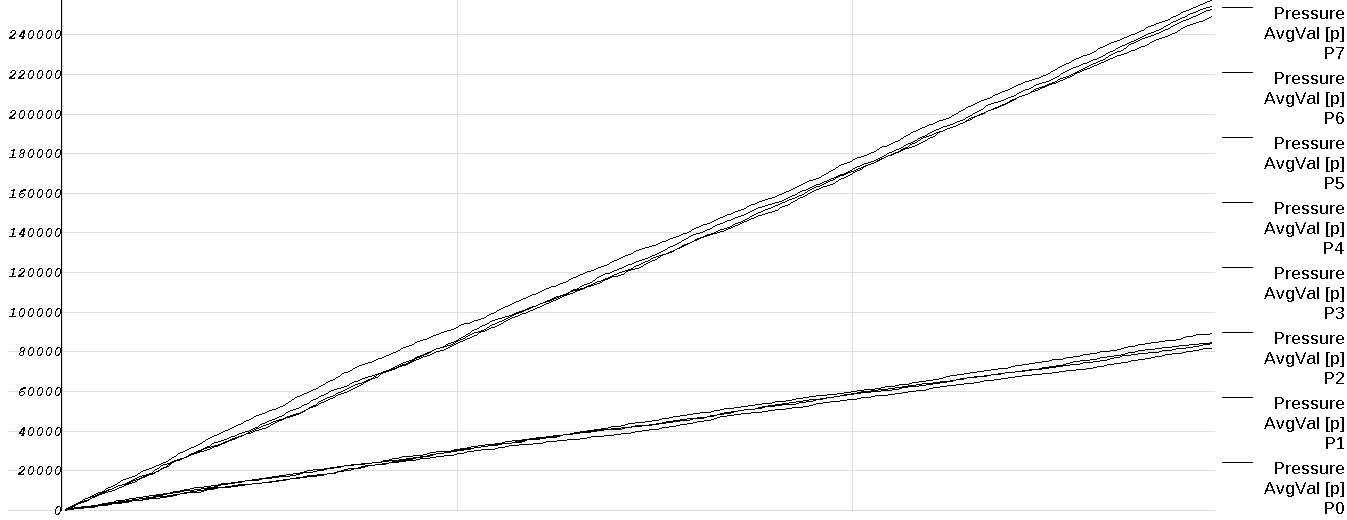
\includegraphics[width=15cm]{chart_pressure.png}
\end{figure}

\clearpage

\begin{comment}
%bulletlist
\paragraph\noindent\textbf{Overview of the linear program}
\begin{itemize}
\renewcommand{\labelitemi}{$\bullet$}
\item Load image from disk
\item Calculate average RGB sum
\item Calculate output image
\item Write image to disk
\end{itemize}

%picture import
\begin{figure}[!h]
  \caption{Run times related to number of cores for the different images.}
  \label{runtime_vs_cores}
  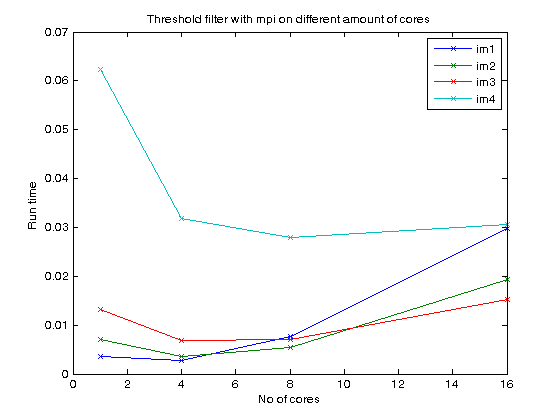
\includegraphics[scale=0.9]{../plots/runtimevscoresthres.png}
\end{figure}

%table
\begin{table}[h!]
  \caption{$MPixels/Second$ when running with different amount of threads and on different data.}
  \label{mpixelspersecond}
  \begin{tabular}[h]{|l|l|l|l|l|l|}
    \hline
                      & 1      & 2      & 4      & 8      & 16\\
    \hline
    im1.ppm           & 135.41 & 183.31 & 184.94 & 68.89  & 21.77\\ 
    im2.ppm           & 150.01 & 209.17 & 274.71 & 201.65 & 63.15\\ 
    im3.ppm           & 146.25 & 209.72 & 274.44 & 275.62 & 138.23\\ 
    im4.ppm           & 145.07 & 212.56 & 286.41 & 332.90 & 297.42\\
    \hline
  \end{tabular}
\end{table}

%citation from bibliography
\cite{fenwick}

%bibliography
\clearpage
\begin{thebibliography}{9}
  \bibitem{fenwick}
    Binary Indexed Trees,
    \emph{Algortihmist}.\\
    \url{http://community.topcoder.com/tc?module=Static\&d1=tutorials\&d2=binaryIndexedTrees}
  \bibitem{ppm}
    Mark Nelson,
    \emph{Arithmetic Coding + Statistical Modeling = Data Compression}, 1991.\\
    \url{http://marknelson.us/1991/02/01/arithmetic-coding-statistical-modeling-data-compression/}
  \bibitem{ppmc}
    PPM
    \url{http://www.cs.ucf.edu/courses/cap5015/ppm.pdf}

\end{thebibliography}a

%sourcecode listing
\lstinputlisting[caption=mpiblur.c]{../mpiblur.c}
\end{comment}

\clearpage
\section{Source code}

\lstinputlisting[caption=simulate.c]{../lab4/simulate.c}
\clearpage
\end{document}
